\documentclass[12pt,titlepage]{article}

\usepackage{float}
\usepackage[T1]{fontenc}
\usepackage[utf8]{inputenc}
%\usepackage[square,numbers]{natbib}
\usepackage{amsmath}
\usepackage{amssymb}
\usepackage[top=1.5cm, bottom=1.5cm, left=1.5cm, right=1.5cm]{geometry}
\usepackage{graphicx}
\usepackage{float}
\usepackage{multicol}
\usepackage{lipsum}
\usepackage{ragged2e}
\usepackage{eurosym}
\usepackage{indentfirst}
\usepackage{minted}
\usepackage{titlesec}
\usepackage{pifont}
\usepackage{url}
\usepackage{epsf}

\usepackage[utf8]{inputenc}
\usepackage{color}
\usepackage{multicol}
\usepackage{graphicx}
\usepackage{animate}
\usepackage{subfigure,color,soul}

\usepackage{array, multirow, makecell}
\setcellgapes{1pt}
\makegapedcells
\newcolumntype{R}[1]{>{\centering\arraybackslash }b{#1}}
\newcolumntype{L}[1]{>{\centering\arraybackslash }b{#1}}
\newcolumntype{C}[1]{>{\centering\arraybackslash }b{#1}}

\usepackage{stmaryrd}
\usepackage{dsfont}
\usepackage{amsmath}
\usepackage{xcolor}         % pour d\'efinir plus de couleurs
\usepackage{animate}
\usepackage{ulem}
\usepackage{url}
%\usepackage{multimedia}
\usepackage{geometry}

\usepackage[english,french]{babel}
\usepackage{hyperref}
\usepackage[T1]{fontenc}
\usepackage{blindtext}

\newcommand{\itemmarker}{{\small\textbullet}}
\newcommand{\ratingmarker}{\faCircle}

\numberwithin{figure}{subsubsection} % Commande de BibiFlo pour faire des trucs super géniaux qui pètent leur race dans LOF

\numberwithin{table}{subsubsection}

\usepackage{nomencl} 
\makenomenclature 
\renewcommand{\nomname}{Liste des abréviations}% Pour redéfinir le titre De cette liste

\usepackage[style=ieee,]{biblatex}
\addbibresource{RapportDeStage.bib}
\renewcommand{\refname}{Bibliographie et sources}


%________________________________________________________________________________________________%

\begin{document}

\begin{titlepage}
\newcommand{\HRule}{\rule{\linewidth}{0.5mm}}
\center
\textsc{\LARGE
Université de Nantes\\[0.1cm]
Faculté de Sciences et Techniques\\[0.4cm]
Licence 3 Sciences Pour l'Ingénieur
} \\[0.6cm]
\HRule \\[0.4cm]
{ \huge \bfseries Rapport de stage :\\
                Mise en place d'un atelier\\
                de fabrication d'une main robotisée }\\[0.4cm]
\HRule \\[1.5cm]
\textbf{\LARGE Albaladejo Joris}
\\[0.5cm]
\Large 4 Janvier 2021\\
    -\\
    26 Février 2021 \\ [0.5cm]

\textsc{\LARGE Association 1901 \textit{Robots !}}\\
             \url{https://www.association-robots.com/}\\[1cm]
             \LARGE Tutrice : \LARGE Noémie Spiessert\\
             \LARGE Fonction : Responsable Opérationnelle\\[1cm]
             \RaggedRight
             
\includegraphics[width=250pt]{images main/logo_univ_nantes.jpg}
             \hspace{2cm}
             
\includegraphics[width=150pt]{images main/logo_asso.png}
\end{titlepage}



%________________________________________________________________________________________________%

\tableofcontents

\newpage

\listoffigures

\newpage

\listoftables

\newpage

\nomenclature{\textbf{CAO}}{Conception Assistée par Ordinateur}
\nomenclature{\textbf{CAD}}{Computer Aided Design}
\nomenclature{\textbf{TSA}}{Trouble du Spectre Autistique}
\nomenclature{\textbf{Kg}}{Kilogramme}
\nomenclature{\textbf{ECV}}{\'Ecole de Communication Visuelle}
\nomenclature{\textbf{CHU}}{Centre Hospitalier Universitaire}
\nomenclature{\textbf{LS2N}}{Laboratoire des Sciences du Numérique de Nantes}
\nomenclature{\textbf{IMT}}{Institut Mines-Télécom}
\nomenclature{\textbf{MOOC}}{Massive Open Online Course}
\nomenclature{\textbf{FUN}}{France Université Numérique}
\nomenclature{\textbf{V}}{Volts}
\nomenclature{\textbf{PLA}}{Polylactic Acid}
\nomenclature{\textbf{3D}}{ 3 Dimensions}
\nomenclature{\textbf{PCB}}{Printed Circuit Board}

\printnomenclature

\newpage
%________________________________________________________________________________________________%

\begin{flushleft}
    \textbf{\LARGE Remerciements}
\end{flushleft}

\vspace{1cm}
En préambule je tiens à remercier Mme Sophie Sakka -- fondatrice de \textit{Robots !} -- et Mme Noémie Spiessert -- Responsable Opérationnelle -- qui m'ont accueilli au sein de l'association et permis de réaliser un stage en accord avec mon projet professionnel. Leur encadrement m'a permis de mener à bien ce projet malgré le délai de 2 mois, correspondant à la durée du stage. 

\vspace{0.5cm}
Merci à M. Zaki Jawhari (Société \textit{URBANDRONE}) d'avoir mis à ma disposition son imprimante \textbf{3D} sans laquelle je n'aurais jamais pu réaliser mon prototype ni mettre en place mon atelier. Merci également pour ses conseils, qui m'ont permis de prendre en main plus rapidement l'imprimante.

\vspace{0.5cm}
Merci également à M. Xavier Laufenberg (Service civique au sein de \textit{Robots !}) pour son aide lors de ma prise en main de l'impression \textbf{3D} et pour son travail de communication autour du projet auprès du public.

\vspace{0.5cm}
Merci à M. Joris L'hotellier (Société \textit{Futon Production}) pour avoir réalisé une vidéo de présentation du projet pour la communication.

\vspace{0.5cm}
Merci à M. Isaac Gutièrrez Payàn qui m'a aidé à préparer et encadrer mon atelier. 

\vspace{0.5cm}
Enfin, j'aimerais dire merci à toute l'équipe de l'association, M. Xavier Robion, M. Philippe Pateau, Mme Laure Vallès Bemelmans, Mme Caroline Gressel ainsi que tous les autres bénévoles que j'ai pu cotoyer pour m'avoir intégré à l'association le temps de mon stage. Nos discussions et leurs suggestions m'auront permis d'aborder au mieux les différentes étapes de la mise en place de l'atelier.

\vspace{0.5cm}
Merci à M. Yannick Aoustin qui m'a encouragé à me challenger en acceptant ce projet. 

\vspace{0.5cm}
Ce stage m’aura permis  de me conforter dans mon choix de projet professionnel, mais également d’acquérir des compétences en gestion de projet et aussi des compétences pour transmettre mes connaissances en réalisant une formation.
\newpage
%________________________________________________________________________________________________%

\section{Introduction}

\begin{center}
\textit{\LARGE ``Un robot n'est pas tout à fait une machine. Un robot est une machine fabriquée pour imiter de son mieux l'être humain.``} 

\huge Isaac Asimov, \textit{La cité des robots}
\end{center}

\vspace{0.8cm}
Dans le cadre de ma Licence 3 Sciences Pour l'Ingénieur parcours \'Electronique, \'Energie électrique et Automatique j'ai réalisé un stage de 8 semaines au sein de l'association 1901 \textit{Robots !}. J'ai souhaité faire mon stage au sein de cette association car j'ai pour projet professionnel de travailler en tant qu'ingénieur biomédical dans le domaine de la conception de prothèses robotisées destinées aux personnes souffrant de handicap. Bien que ce domaine ne soit pas directement lié aux différents projets encadrés par l'association, j'ai notamment été séduit par les différents projets qu'elle entreprend. Ici, le robot n'est pas le centre de l'attention mais c'est bien l'humain qui apprend à utiliser le robot pour améliorer son quotidien.


\vspace{0.5cm}
Pour intégrer l'équipe tout en me rapprochant de mon objectif professionnel et en restant dans l'esprit de l'association, Sophie Sakka m'a proposé de mettre en place un projet spécifique : un atelier de fabrication et de programmation d'une prothèse robotisée. Toutefois, la contrainte du temps mais aussi le fait que mon atelier devait pouvoir s'adresser au grand public m'ont fait pencher pour une main robotisée plutôt qu'une prothèse. L'atelier que j'ai mis en place avait donc pour but de sensibiliser les personnes à la \textbf{CAO} (ou \textbf{CAD} en anglais), à l'impression \textbf{3D}, à l'électronique et à la programmation.


\vspace{0.5cm}
Durant ces 8 semaines, j'ai mis en place un atelier de fabrication de main robotisée accessible à tous. Au delà de la fabrication du prototype de main, la finalité était que je puisse animer cet atelier durant ma dernière semaine de stage. La durée de cet atelier était de 4 demi-journées réparties du lundi 22 Février au jeudi 25 Février.


\vspace{0.5cm}
Dans un premier temps je rappellerai l'histoire de l'association. En seconde partie, j'aborderai les différentes missions que j'ai eu à réaliser pour mettre en place mon atelier. Enfin, je conlurai sur ce que ce stage m'a apporté et j'évoquerai différentes perspectives d'améliorations envisageables pour ce projet.

\newpage
%________________________________________________________________________________________________%

\section{Présentation de \textit{Robots!}}

\subsection{Historique}
\textit{Robots!} \cite{noauthor_association_nodate} est une association déclarée d'intérêt général à but non lucratif. Elle a été crée en Mars 2014 par Sophie Sakka. Elle a au départ eu une démarche orientée autour de la robotique et de l'art. Celle ci a été initiée par Sophie Sakka et Marie Rebérat qui avait pour l'occasion conçu des tenues pour les robots Nao. \`A la suite d'une conférence animée par Sophie Sakka, Xavier Robion, enseignant à l'\textbf{ECV} Nantes, a proposé son aide pour trouver l'identité visuelle de l'association. Le logo présent sur la première page de mon rapport a donc été fait en 2014 par Lucie Crison, une élève de l'\textbf{ECV}. 

\vspace{0.5cm}
Suite aux différentes interventions de Sophie Sakka qui montraient les bienfaits que pouvaient avoir les robots sur les humains, une connexion s'est faite avec le \textbf{CHU} de Nantes. Ainsi le projet \textit{Rob'Autisme} est né d'une reflexion entre Sophie Sakka et Renald Gaboriau, ortophoniste au \textbf{CHU} et encadrant du projet entre 2014 et 2017. Il a également mené une thèse sur le sujet, qu'il a soutenu le 24 septembre 2020 pour obtenir le grade de Docteur du Laboratoire des Sciences du Numérique de Nantes (\textbf{LS2N}).

\subsection{Ses collaborateurs}
Depuis sa création, l'association a eu de nombreux partenaires tels que le CHU de Nantes, le \textbf{LS2N} ou encore l'\'Ecole Centrale de Nantes. Ci-dessous, le détail des partenaires qu'elle a eu depuis sa création.

\begin{figure}[!h]
    \centering
    
\includegraphics[width=300pt]{Partie II/images/partenaires1.PNG}
    
\includegraphics[width=300pt]{Partie II/images/partenaires2.PNG}
    \caption[\, \, Partenaires]{Les partenaires de l'association}
    \label{fig_2.2.0.1}
\end{figure}

%provisoire
\newpage

\subsection{Ses missions}
L'association diffuse un savoir sur les robots et sur leur utilisation auprès du grand public et mène une réflexion sociétale sur comment, dès aujourd'hui, les robots peuvent améliorer notre quotidien. Les bénévoles y mènent différents projets ouverts dès l'âge de 10 ans :

\begin{itemize}
    \item \textit{Rob'Autisme}, un projet se déroulant sur 2 ans pouvant accueillir 6 adolescents de 11 à 16 ans atteints de \textbf{TSA}. Il a pour but de réaliser un accompagnement thérapeutique basé sur l'utilisation des robots Nao (\textit{SoftBank Robotics}) pour permettre aux participants de renforcer leur habileté sociale.
    \item Des ateliers de découvertes et d'initiation à la programmation avec les robots Nao et Thymio (\textit{Mobsya}).
    \item Des stages performances avec Nao et Thymio pour programmer et créer une histoire.
\end{itemize}

%________________________________________________________________________________________________%

\subsection{Positionnement}

\subsubsection{Organisation de l'association}
Depuis sa création en 2014 \textit{Robots !} est présidée par Sophie Sakka, et compte chaque année une cinquantaine d'adhérents.
\begin{figure}[!h]
    \centering
    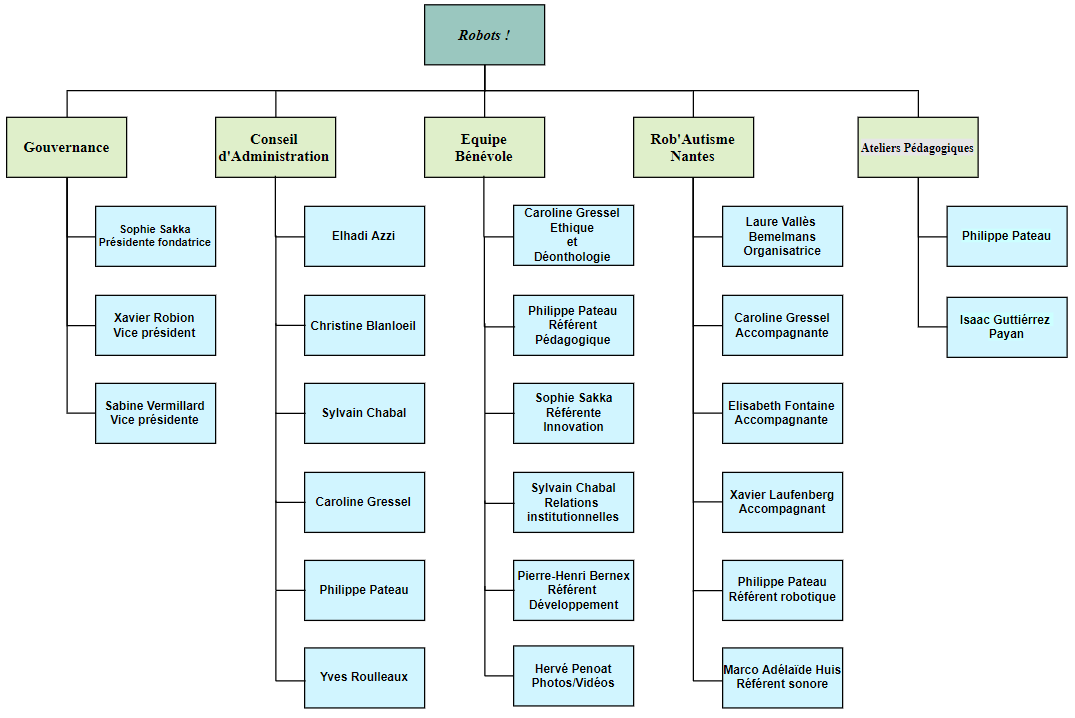
\includegraphics[height=350pt]{Partie II/images/ROBOTS.PNG}
    \caption{\, \, Organisation de \textit{Robots!}}
    \label{fig_3.1.0.1}
\end{figure}

\newpage

\subsubsection{Positionnement au sein de l'association}
Lors de mon stage j'ai intégré l'équipe en charge des ateliers pédagogiques, afin de pouvoir préparer puis animer mon atelier \textit{Montage et programmation d'une main robotisée}.

\begin{figure}[!h]
    \centering
    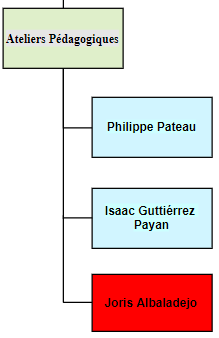
\includegraphics[width=125pt]{Partie II/images/MonPositionnement.PNG}
    \caption{\, \, Mon positionnement au sein de \textit{Robots!}}
    \label{fig_3.2.0.1}
\end{figure}

%________________________________________________________________________________________________%

\section{Mon projet}

La mise en place de mon projet est passée par plusieurs étapes. Il a fallu dans un premier temps que je décide de la manière dont j'allais organiser l'avancement de celui-ci et en élaborant un cahier des charges. Par la suite j'ai entrepris une phase de recherche pour me renseigner sur les différents types de mains robotisées existants ainsi que leur fonctionnement. 

\vspace{0.5cm}
Mes recherches terminées, j'ai commencé les tests sur l'imprimante \textbf{3D} afin d'ajuster le réglage des paramètres pour trouver ceux étant les plus optimaux au vu des contraintes non seulement de temps pour la réalisation du prototype et des pièces nécessaires à l'atelier, mais également la contrainte de solidité à laquelle devait répondre la main. En parallèle de cela, j'ai conçu un code visant à contrôler le mouvement de la main à l'aide de potentiomètres.

\vspace{0.5cm}
Simultanément j'ai engagé la rédaction du manuel d'utilisation de mon atelier afin, d'une-part : de regrouper les connaissances nécessaires à la fabrication de la main, et d'autre-part de manière plus générale, indiquer les ressources permettant de s'initier à la programmation, la \textbf{CAO} et l'impression \textbf{3D}. Enfin, le développement de l'imagination par l'utilisation des robots étant une des valeurs de l'Association, j'ai ouvert des perspectives aux futurs utilisateurs pour qu'ils puissent trouver des solutions correspondants à leurs propres attentes vis à vis de cette main. 

%provisoire
\newpage

\subsection{La préparation en amont}
\subsubsection{La phase de recherche}
Au départ Sophie Sakka m'avait proposé de mettre en place un atelier de fabrication de prothèse robotisée. Cepedant, après réflexion j'en ai conclu qu'une prothèse serait compliquée à faire en raison des connaissances nécessaires, de la nécessité que l'atelier final doit être réalisable par des personnes non spécialistes dans ce domaine et de la contrainte de la durée de mon stage qui était de deux mois. J'ai donc décidé de m'orienter plutôt vers une main robotisée. 

\vspace{0.5cm}
Pour appuyer ma décision je l'ai formalisée à l'aide du tableau comparatif suivant :

\begin{table}[!h]
    \centering
    \begin{tabular}{|c|c|c|}
        \hline Caractéristiques & Main robotisée & Prothèse robotisée  \\
         \hline Capteurs sensoriels & Pas obligatoire & Obligatoire \\
         \hline Matériaux adaptés à la peau & Pas nécessaire & Obligatoire \\
         \hline Poids (Moyenne depuis 2010) & Moins de 1Kg & Moins de 1Kg \\
         \hline Autonomie & Dépend de l'alimentation & environ 1 journée \\
         \hline Fonctionnement & Code informatique & Signaux électriques nerveux \\
         \hline
    \end{tabular}
    \caption[\, \, Comparaison Main robotisée/Prothèse robotisée]{Tableau comparatif Main robotisée/Prothèse robotisée}
    \label{tab_4.1.1.1}
\end{table}

Après avoir effectué mon travail de recherches génériques sur les mains robotisées, j'ai commencé à chercher un modèle de mains en fichiers \textbf{3D} libre de droit et correspondant à mes attentes, pour l'imprimer. J'ai donc axé mes recherches sur les mains robotiques, et j'ai découvert un projet sur le site \textit{Instructables}. Ce projet était une main imprimée en \textbf{3D} contrôlée en bluetooth via un smartphone réalisée par un utilisateur nommé \textit{TechMartian}\cite{techmartian_3d_nodate}.

\vspace{0.5cm}
Bien que ce projet soit en libre accès sur le site, je l'ai contacté pour lui expliquer ma démarche, malheureusement il ne m'a pas répondu.

\vspace{0.5cm}
Au fil de mes recherches, je suis donc arrivé aux résultats suivants :
\begin{table}[!h]
    \centering
    \begin{tabular}{|c|c|}
       \hline Ce que l'on trouve facilement  & Ce que l'on a du mal à trouver \\
        \hline Des modèles de mains robotiques pour l'impression \textbf{3D} & Des modèles avec des dimensions \\  & proches de celles d'une vraie main \\
        \hline Le type d'actions que doit pouvoir effectuer la main choisie & Des articles accessibles au grand public \\
        \hline Des projets de mains robots réalisés par des particuliers & Les composants exacts utilisés\\
         & sur les modèles trouvés \\
        \hline
    \end{tabular}
    \caption{\, \, Résultats de la documentation}
    \label{tab_4.1.1.2}
\end{table}

%provisoire
\newpage

J'ai observé que le fait d'ouvrir une pièce \textbf{3D} avec un logiciel différent de celui qu'avait utilisé le créateur de la pièce pouvait en effet générer des problèmes au niveau des dimensions des pièces. Toutefois, ce problème peut-être évité si l'on trouve un modèle conçu sur le même logiciel que celui que l'on utilise, ou bien en effectuant une modification de l'échelle lors de la préparation de l'impression sur le trancheur \textbf{3D}.

\vspace{0.5cm}
Une fois trouvé mon modèle de main à imprimer en \textbf{3D}, je me suis attelé à l'observation de la différence des mouvements que pouvaient effectuer une main humaine et la main robotique que j'allais monter. J'ai donc pris la décision de réaliser des modélisations cinématiques pour observer les différences entre les deux types de main.
Ci-dessous, la modélisation d'une main humaine en m'inspirant de celle vue dans la thèse de Giulio Cerruti \cite{cerruti_design_2016}, ainsi que celle de la main robotique que j'ai décidé d'utiliser pour mon atelier.

\begin{figure}[!h]
    \centering
    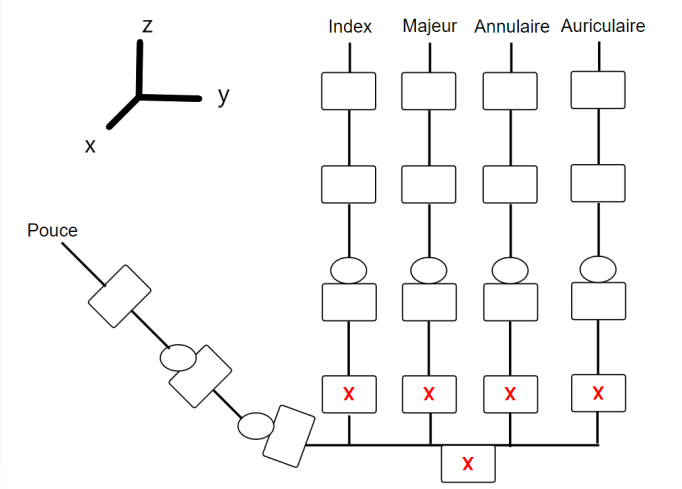
\includegraphics[width=250pt]{Partie II/images/modé_ciné_main humaine.PNG}
    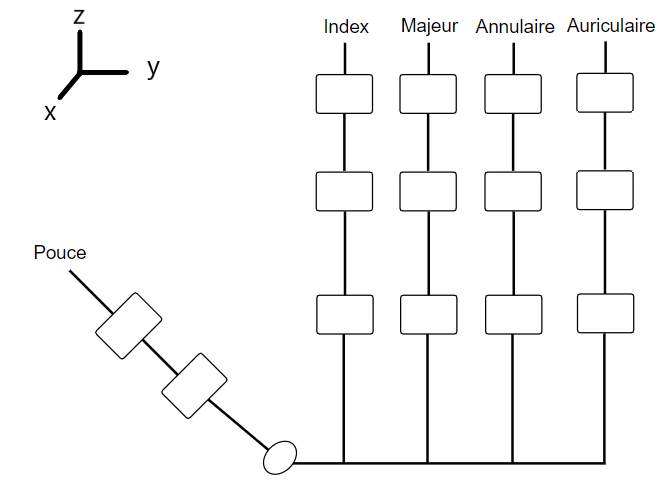
\includegraphics[width=250pt]{Partie II/images/modé_ciné_main_rob.PNG}
    \caption[\, \, Modélisations cinématiques]{\centering Modélisations cinématiques d'une main humaine (à gauche) \\ \centering et de ma main robotisée (à droite)}
    \label{fig_4.1.1.1}
\end{figure}

\begin{flushleft}
    \underline{\textit{\large Légende :}}
\end{flushleft}

\begin{itemize}
    \item ovales : rotation autour de l'axe z
    \item rectangles : rotation autour de l'axe y
    \item rectangles avec une croix rouge : degré de liberté négligé
\end{itemize}

%provisoire
\newpage

\subsubsection{La phase d'organisation}
Une fois ma phase de recherche terminée, j'avais les fichiers nécessaires pour l'impression du modèle \textbf{3D}. J'ai donc pu établir un cahier des charges et un planning prévisionnel pour mon projet, afin de pouvoir comparer à la fin si mes prévisions étaient les bonnes ou pas.

\vspace{0.5cm}
Ici, le tableau comparatif de mon planning prévisionnel et du temps réel que j'ai passé  sur les différentes tâches :

\begin{table}[!h]
    \centering
    \begin{tabular}{|c|c|c|}
        \hline Tâches & Temps passé prévu & Temps passé réel \\
        \hline Documentation sur les mains robotisées & 25h & 30h \\
        \hline Recherche et sélection du modèle \textbf{3D} à imprimer & 6h & 9h \\
        \hline Choix/commande/test du matériel nécessaire & 4h & 10h \\
        \hline \'Etablissement du cahier des charges & 3h & 3h \\
        \hline Documentation sur l'impression \textbf{3D} & 15h & 12h \\
        \hline Impression des pièces (pour le prototype et l'atelier) & 50h & 70h \\
        \hline Réalisation et test du code Arduino & 10h & 5h \\
        \hline Préparation de l'atelier & 40h & 65h \\
        \hline communication autour de l'atelier & 30h & 25h \\
        \hline Animation de l'atelier & 16h & 16h \\
        \hline
    \end{tabular}
    \caption[\, \, Planning]{Comparaison du planning prévisionnel et du temps réel passé sur les tâches}
    \label{tab_4.1.2.1}
\end{table}

Ci-dessous, le cahier des charges du projet.

\begin{table}[!h]
    \centering
    \begin{tabular}{|l|l|}
        \hline Contexte & Mise en place d'un atelier de formation "loisir" \\
         & de fabrication d’une main robotique en impression \textbf{3D}. \\
        \hline Positionnement & On se place dans le cas de la création d'une main robotisée. \\
        \hline Objectif & Animer un atelier de formation grand public. \\
         & Chaque participant doit repartir avec sa main. \\
        \hline Besoins Fonctionnels & La main doit être capable de tenir un objet léger. \\
         & La formation finale doit être adaptée au grand public. \\
        \hline
    \end{tabular}
    \caption{\, \, Cahier des charges du projet}
    \label{tab_4.1.2.2}
\end{table}

%provisoire
\newpage

\subsubsection{L'achat du matériel}
Après avoir réalisé mon cahier des charges et établi mon planning, je me suis penché sur la commande du matériel nécessaire à la réalisation du prototype et l'animation de l'atelier. Nous avions convenu qu'il y aurait 6 places, je devais donc prévoir la fabrication de 7 mains.

\begin{table}[!h]
    \centering
    \begin{tabular}{|l|l|l|l|l|}
        \hline Objet & Quantité/main & Prix/Unité & Quantité commandée & coût total\\
        \hline Carte Arduino \textit{Uno} & 1 pièce & $14.90$\euro{} & 7 pièces & $124.20$\euro{}\\
        \hline Câble Dupont mâle-mâle & 32 pièces & $0.065$\euro{} & 2*120 pièces & $15.76$\euro{}\\
        \hline Platine d'essai & 1 pièce & $4.99$\euro{} & 7 pièces & $34.93$\euro{}\\
        \hline Potentiomètre linéaire 10k$\Omega$ & 5 pièces & $1$\euro{} & 35 pièces & $35$\euro{}\\
        \hline pile 9V & 1 pièce & $3$\euro{} & 7 pièces & $21$\euro{}\\
        \hline support de pile & 1 pièce & $2.99$\euro{} & 7 pièces & $20.93$\euro{}\\
        \hline Servomoteur SG90 9g & 5 pièces & $1.39$\euro{} & 4*10 pièces & $55.56$\euro{}\\
        \hline Coût total & & $40$\euro{} & & $307.38$\euro{} \\
        \hline
    \end{tabular}
    \caption{\, \, Matériel nécessaire au fonctionnement de la main}
    \label{tab_4.1.3.1}
\end{table}

J'ai également dressé une liste du matériel commun nécessaire au montage des 7 mains prévues :
\begin{itemize}
    \item Des vis pour fixer le support des servomoteurs sur le bras et pour fixer les poulies sur les servomoteurs
    \item Une bobine de câble élastique pour les articulations
    \item Une bobine de câble métallique pour tirer les doigts avec les servomoteurs
    \item Un pistolet à colle chaude
    \item Une bobine de filament \textbf{PLA} de couleur noire pour l'impression \textbf{3D}
    \item Une bobine de filament \textbf{PLA} de couleur verte pour l'impression \textbf{3D}
\end{itemize}

\vspace{0.5cm}
Nous avions déjà le pistolet à colle et nous n'avons donc pas eu à l'acheter. Les vis quand à elles étaient présentes dans les sachets individuels de chaque servomoteur. Ci-dessous, un tableau dressant le total du coût d'achat du matériel :

\begin{table}[!h]
    \centering
    \begin{tabular}{|c|c|c|}
        \hline Matériel & quantité achetée & prix \\
        \hline Bobine de câble élastique & 1 & $7.9$\euro{} \\
        \hline Bobine de câble métallique & 1 & $2$\euro{} \\
        \hline Bobine de filament \textbf{PLA} & 2 & 2*$19.90$\euro{}\\
        \hline
    \end{tabular}
    \caption{\, \, Matériel commun à la fabrication des 7 mains}
    \label{tab_4.1.3.2}
\end{table}

%provisoire
\newpage

\subsubsection{La communication}

Une fois tout le matériel choisi et commandé, j'ai pu discuter avec les différents membres de \textit{Robots!} pour décider de quelle manière nous allions communiquer pour promouvoir l'atelier. Nous avons demandé à Joris L'hotellier de réaliser un petit clip vidéo (disponible en \textbf{annexe 1}) que l'on puisse diffuser sur différents réseaux sociaux (Facebook, LinkedIn) lors de l'annonce de l'atelier.

\vspace{0.5cm}
Pour promouvoir l'atelier j'ai donc rédigé un petit texte expliquant ce dont il allait être question, et nous l'avons accompagné de la vidéo. Noémie Spiessert s'est occupée de la diffusion de celui-ci sur les différents réseaux de l'association, que nous repartagions ensuite sur nos comptes personnels. Elle a également ouvert les inscriptions au public via le site \textit{helloasso}.

\vspace{0.5cm}
Pendant ce temps, Xavier Laufenberg a de son côté conçu un flyer (disponible en \textbf{annexe 2}) expliquant le contenu de l'atelier. Nous sommes ensuite allés le faire imprimer en plusieurs exemplaires pour le distribuer dans des commerces de la ville.

\vspace{0.5cm}
La diversité de notre communication, que cela soit les flyers ou les posts sur les différents réseaux nous a permis d'obtenir 4 inscriptions à l'atelier en moins d'une semaine malgré les contraintes sanitaires ! Les 2 dernières places n'ont malheureusement pas été remplies, toutefois c'était un challenge de plus de relevé.

\vspace{0.5cm}
En effet, s'il était prévu que j'anime quoi qu'il arrive un atelier durant ma dernière semaine de stage, nous avions peur qu'au vu des circonstances actuelles peu de personnes soient interéssées et que je ne l'anime pas auprès d'un véritable public mais auprès de membres de l'association.

\subsubsection{La rédaction du manuel d'utilisation de l'atelier}

Afin de préparer mon atelier \textit{Montage et programmation d'une main robotisée} j'ai rédigé un manuel d'utilisation (disponible en \textbf{annexe 3}). Ce manuel avait pour but de visualiser la manière dont j'allais structurer mon atelier, tout en expliquant à chaque participant de manière assez simple le fonctionnement des composants, de la main, mais aussi où trouver les ressources pour faire de l'impression \textbf{3D} et trouver des modèles de \textbf{CAO}. 

\vspace{0.5cm}
Au-delà de la rédaction, cela m'a demandé un travail de réflexion sur comment j'allais présenter toutes les notions, et un travail de documentation supplémentaire, par exemple sur les différentes structures proposant un service d'impression \textbf{3D} à Nantes.

\vspace{0.5cm}
Il était également destiné à être disponible en accès libre sur le site de \textit{Robots!}. Par conséquent, il devait être suffisamment complet et détaillé pour qu'une personne souhaitant reproduire le projet en autonomie ait toutes les clefs en main pour se former de la même manière qu'une personne ayant assisté à l'atelier.

%provisoire
\newpage

\subsection{La partie technique}
\subsubsection{L'impression 3D}

J'ai commencé la partie technique en m'occupant de l'impression \textbf{3D} car c'était la première fois que j'utilisais une imprimante \textbf{3D}. Je me suis donc renseigné en lisant le manuel d'utilisation \cite{anycubic_usuer_nodate} pour me familiariser avec les mesures de sécurité, ainsi que les caractéristiques de l'imprimante. Cette imprimante était la \textit{Chiron} de chez \textit{Anycubic}.

\vspace{0.5cm}
Une fois l'installlation et la prise en main du logiciel \textit{Ultimaker Cura} \cite{noauthor_ultimaker_nodate} réalisées, j'ai utilisé ce trancheur \textbf{3D} pour réaliser mes impressions. Une fois tout cela fait, j'ai alors enfin pu réaliser des tests pour trouver les paramètres qui convenaient le mieux pour mon projet (Voir en \textbf{annexe 4} les photos de quelques tests que j'ai réalisé, ainsi que du résultat avec les paramètres finaux). J'ai donc créé un profil \textit{Cura} spécifique pour ne pas avoir à modifier les réglages à chaque nouvelle impression (Voir ci-dessous).

\vspace{0.5cm}
\begin{table}[!h]
    \centering
    \begin{tabular}{|l|l|l|}
        \hline Catégorie & Nom du paramètre & Valeur\\
        \hline Qualité & Hauteur de la couche & 0.3 mm\\
        \hline Coque & \'Epaisseur de la paroi & 0.5 mm\\
        \hline & Nombre de lignes de la paroi & 1\\
        \hline & \'Epaisseur du dessus/dessous & 0.8 mm\\
        \hline & \'Epaisseur du dessus & 0.8 mm\\
        \hline & Couche supérieure & 3\\
        \hline & \'Epaisseur du dessous & 0.8 mm\\
        \hline & Couche inférieure & 3\\
        \hline & Expansion horizontale & 0 mm\\
        \hline Remplissage & Densité du remplissage & 5\% \\
        \hline & Motif de remplissage & Grille\\
        \hline Matériau & Température d'impression & 200°C\\
        \hline & Température du plateau & 85°C\\
        \hline Vitesse & Vitesse d'impression & 80mm/s\\
        \hline Déplacement & Activer la rétraction & Oui\\
        \hline Refroidissement & Activer le refroidissement de l'impression & Oui\\
        \hline & Vitesse du ventilateur & 100\% \\
        \hline Supports & Générer les supports & Non \\
        \hline Adhérence du plateau & Type d'adhérence du plateau & Bordure \\
        \hline
    \end{tabular}
    \caption[\, \, Profil d'impression]{Profil d'impression sur \textit{Ultimaker Cura}}
    \label{tab_4.2.1.1}
\end{table}

\vspace{0.5cm}
Pour continuer à me former sur la modélisation et l'impression \textbf{3D} j'ai suivi le \textbf{MOOC} \textit{Imprimer en \textbf{3D}} \cite{imt_imprimer_nodate} organisé par l'\textbf{IMT} Atlantique. Je l'ai suivi via la plateforme \textit{\textbf{FUN} \textbf{MOOC}} et j'ai obtenu une attestion de réussite (disponible en \textbf{annexe 5}).

%provisoire
\newpage

\subsubsection{La programmation du code}

Pour contrôler le mouvement de ma main je souhaitais au départ suivre le principe mis en place par le créateur du projet dont je me servais, à savoir la programmation via Arduino \cite{noauthor_arduino_nodate}. Ceci pour pouvoir gérer le mouvement des doigts en bluetooth à l'aide une application de smartphone. Cependant, la carte qu'il utilisait pour son projet était une carte Arduino \textit{101}, alors que celle que j'utilisais était une Arduino \textit{Uno}.

\vspace{0.5cm}
En effet ces deux cartes sont différentes non seulement de par leur prix, mais également de par leurs fonctionnalités. La \textit{101} comporte un module bluetooth intégré alors que sur la \textit{Uno} ce module doit être acheté séparement. Un de mes challenges était notamment de réduire au maximum le coût de fabrication d'une main, afin de pouvoir proposer l'atelier à un prix raisonnable pour les participants, tout en restant en accord avec les tarifs mis en place par l'association.

\vspace{0.5cm}
De plus la programmation d'un module bluetooth était plus compliquée à mettre en oeuvre et à expliquer à des personnes totalement étrangères à la programmation. J'ai donc pris la décision de m'orienter vers l'utilisation de potentiomètres et de cartes Arduino \textit{Uno} pour optimiser un maximum le coût de fabrication.

\vspace{0.5cm}
J'ai donc écrit un premier code assez simple pour tester rapidement le fonctionnement de chaque servomoteur à la réception de la commande : 

\begin{figure}[!h]
    \centering
    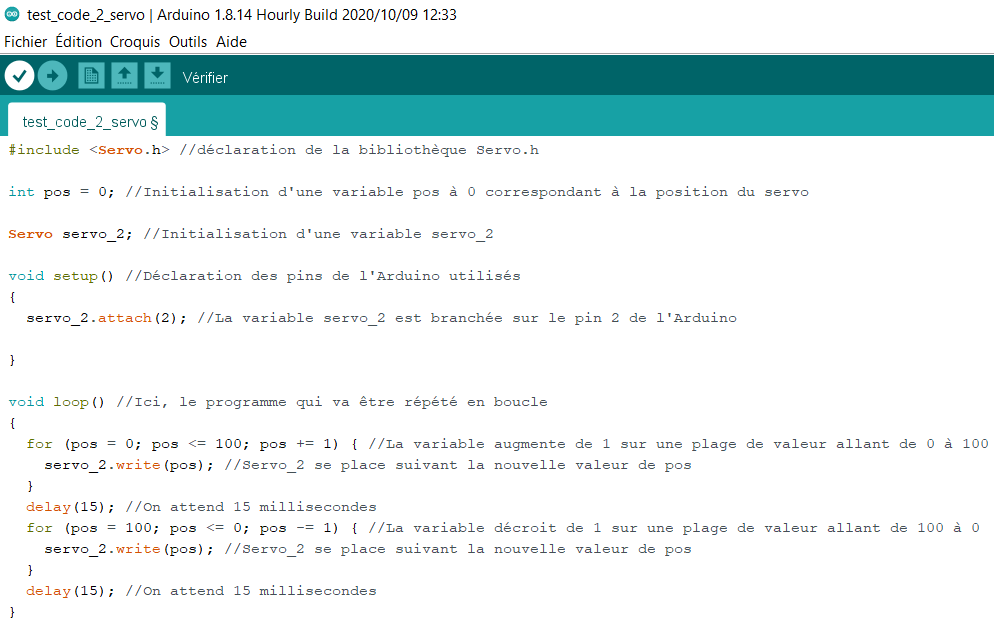
\includegraphics[width=425pt]{Partie II/images/code_test.PNG}
    \caption[\, \, Code de test]{Code de test du fonctionnement des servomoteurs}
    \label{fig_4.2.2.1}
\end{figure}

Vous trouverez en \textbf{annexe 6} une vidéo montrant ce code en fonctionnement.

%provisoire
\newpage

Cependant la main ne devait pas bouger de manière automatique, mais pouvoir être contrôlée manuellement. J'ai donc rédigé un programme permettant de contrôler les 5 servomoteurs indépendemment à l'aide de 5 potentiomètres : 

\begin{figure}[!h]
    \centering
    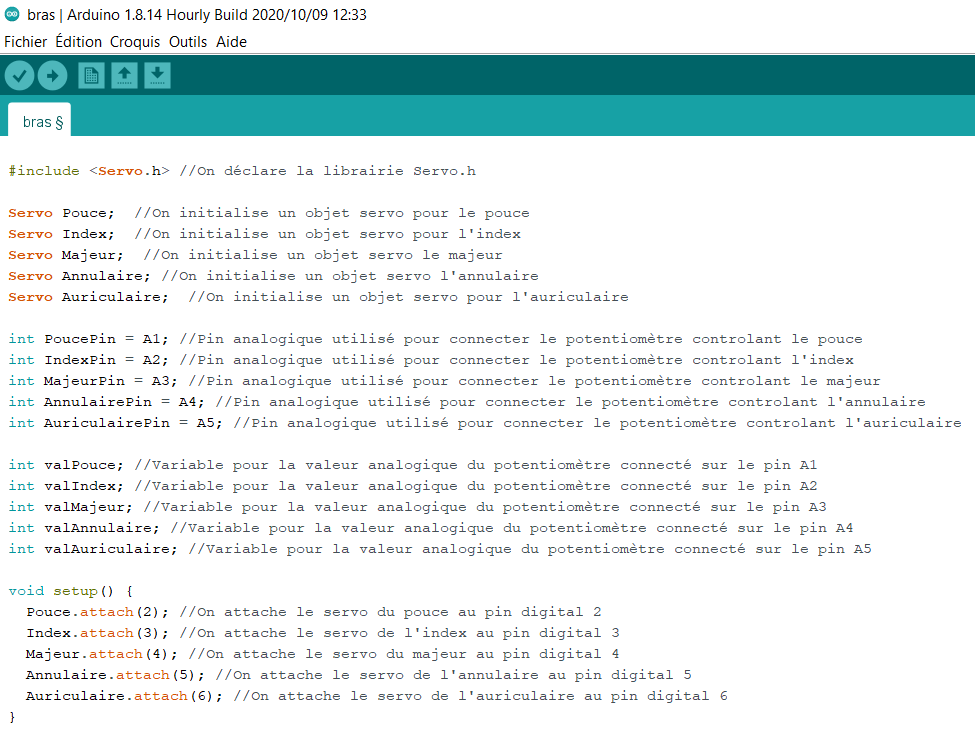
\includegraphics[width=450pt]{Partie II/images/code_bras_1.PNG}
    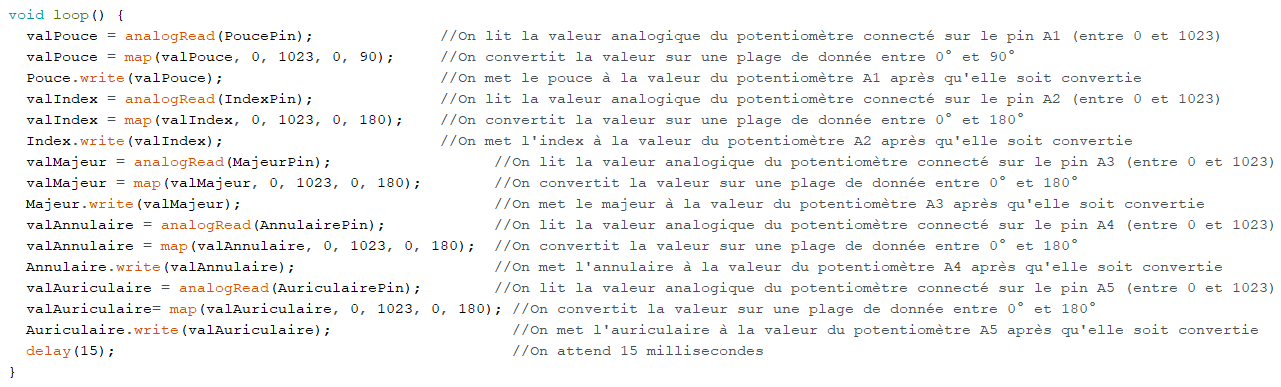
\includegraphics[width=450pt]{Partie II/images/code_bras_2.PNG}
    \caption[\, \, Code de fonctionnement]{Code de fonctionnement de la main}
    \label{fig_4.2.2.2}
\end{figure}

Vous trouverez en \textbf{annexe 7} une vidéo montrant ce code en fonctionnement.

%provisoire
\newpage

\subsection{L'atelier}

\subsubsection{Les problématiques rencontrées}

Pour mettre en place cet atelier, je devais réaliser l'impression de 7 mains. Cependant la durée d'impression des pièces était à première vue une contrainte pour pouvoir être prêt pour ma dernière semaine. Afin de résoudre cette difficulté il était nécessaire d'imprimer plusieurs pièces à la fois. Cela nous contraignait cependant à ne pouvoir lancer qu'une seule impression par jour.

\vspace{0.5cm}
En effet, l'impression de toutes les pièces du projet était affichée comme prenant 9h et 56 minutes et consommait 24.88 mètres de filament \textbf{3D} lorsque nous déposions les pièces sur le plateau virtuel du logiciel. Toutefois ceci était calculé avant le début de l'impression, et il fallait compter environ 2h supplémentaires avant qu'elle soit réellement finie. Ne pouvant pas faire tourner l'imprimante en dehors de nos horaires de présence à l'association pour des questions de sécurité, nous ne pouvions pas imprimer une main entière à chaque fois.

\vspace{0.5cm}
De plus, il arrivait parfois que les pièces se décollent du plateau au cours de l'impression, à cause des changements de température dans la pièce où se situait l'imprimante. Cela exigeait parfois que nous relancions de nouvelles impressions encore moins grosses par manque de temps avant la fin de la journée.

\vspace{0.5cm}
Au-delà du temps d'impression relativement long, il fallait prendre en compte le fait que chaque impression qui échouait plus ou moins loin dans son avancement nous faisait consommer du filament. Ces ratés ajoutés aux tests réalisés pour la prise en main de l'imprimante et du logiciel ont donc nécessité l'achat de plusieurs bobines.

\vspace{0.5cm}
N'ayant jamais animé d'atelier auparavant il a également fallu que je détermine comment j'allais aborder les différentes notions, tout en sachant que lorsque j'ai commencé ma préparation je n'avais pas encore d'inscrit. Je ne savais donc pas si j'allais devoir faire cet atelier à des enfants, des adolescents ou des adultes, expérimentés en programmation et en impression \textbf{3D}, ou non.

\vspace{0.5cm}
Pour compenser cela j'ai donc opté pour la préparation de quelques quizzes via le site \textit{Kahoot} et l'utilisation de quelques vidéos \textit{YouTube} afin de rendre l'apprentissage et la compréhension des notions la moins difficile possibles, tout en apportant un côté ludique qui favorise la mémorisation. J'ai également utilisé le support de cours d'Informatique Industrielle que j'ai suivi à l'université au semestre 1 \cite{cadiou_langage_nodate}, pour expliquer au mieux le fonctionnement de base d'un code Arduino.

\vspace{0.5cm}
Pour la partie pratique, j'ai opté pour un travail collaboratif mais qui permettait de respecter les contraintes sanitaires. Chaque participant avait son matériel, mais je les invitais à intervenir entre eux pour se conseiller et partager leurs idées sur la réalisation de telle ou telle tâche.

%provisoire
\newpage

\subsubsection{Le profil des participants}

La semaine d'atelier démarrait donc avec 4 participants. En leur posant quelques questions le 1er jour j'ai pu établir un profil de chacun d'entre eux, que je présente dans un tableau récapitulatif ci-dessous.

\begin{table}[!h]
    \centering
    \begin{tabular}{|c|c|c|c|}
        \hline Numéro du participant & Âge & Notions en impression \textbf{3D} & Notions en programmation\\
        \hline Participant 1 & 10 ans et demi & Non & Oui\\
        \hline Partcipant 2 & 11 ans & Non & Non\\
        \hline Participant 3 & 14 ans & Non & Non\\
        \hline Participant 4 & 16 ans & Non & Oui\\
        \hline
    \end{tabular}
    \caption[\, \, Profil des participants]{Tableau récapitulatif du profil des participants}
    \label{tab_4.3.2.1}
\end{table}

j'ai trouvé cela intéressant, car le plus jeune et le plus âgé du groupe avaient tous deux quelques notions en progrmmation, mais par deux biais différents. Au final ils avaient d'une certaine manière les mêmes bases. En matière d'impression \textbf{3D} ils étaient tous novices dans ce domaine, ce qui était plus aisé pour en expliquer le fonctionnement. 
\subsubsection{La finalité}

Malgré leurs profils différents chacun d'eux a été intéressé et s'est impliqué pendant l'atelier, et le travail collaboratif leur a permis d'avancer et d'arriver à ce qu'ils montent et programment tous leur main. L'objectif était qu'ils repartent avec des compétences suffisantes pour pouvoir approfondir eux même le projet ou se lancer seuls dans de nouveaux projets, je ne devais donc pas leur apporter une réponse à la moindre difficulté, mais plutôt les aiguiller pour qu'ils trouvent leur propre manière de résoudre le problème qu'ils rencontraient.

\vspace{0.5cm}
Le dernier jour, ils ont chacun pu repartir leur main, et étaient tous contents de ce qu'ils avaient produit. Les parents ont également fait des retours positifs, disant que leurs enfants avaient été très emballés par l'atelier. Certains enfants mêmes envisagent même de revenir à l'association pour participer à de futurs ateliers sur les robots Nao et Thymio !







%________________________________________________________________________________________________%

\newpage

\section{Conclusion}

J'ai eu la chance de mener au cours de ce stage un projet en accord avec mon objectif professionnel. Le fait que Sophie Sakka m'ait proposé de créer cet atelier et de l'encadrer pour l'association m'a permis de découvrir différentes facettes de la gestion de projet, tout en étant encadré et aidé par des personnes dans la réalisation de ces différentes tâches.

\vspace{0.5cm}
Tout cela m'a aidé à visualiser ce qu'étaient les contraintes auxquelles nous devons faire face pour mener à bien un projet dans un délai imparti. Dans ce contexte j'ai réussi à aller au bout de l'objectif, à savoir animer l'atelier durant la dernière semaine. Les 4 personnes inscrites ont toutes pu repartir avec leur propre main et avec, je l'espère, l'envie d'améliorer le projet que j'avais mis en place ou de se lancer seuls dans de nouvelles conceptions robotiques.


\vspace{0.5cm}
Le projet initial prévoyait de pousser la partie électronique un peu plus loin en portant le microcontroleur de l'Arduino \textit{Uno}, les composants nécessaires de la carte et les potentiomètres sur une plaque de \textbf{PCB}. Pour des raisons de complexité, de coût mais également de sécurité, le projet a été revu. En effet, cela incluait d'appprendre aussi aux participants à faire de la soudure et nécessitait donc du matériel et des compétences supplémentaires.

\vspace{0.5cm}
J'ai aussi pris conscience qu'il faut toujours prévoir une marge de manoeuvre lors de la réalisation d'un projet. Certaines tâches peuvent s'avérer plus longues que ce que l'on avait imaginé au départ et il est important de réaliser un planning dès le début. Il peut aussi parfois y avoir des tâches qui prennent du retard sans que cela soit forcément de notre fait (impressions ratées, réception tardives des commandes, etc...) et là encore le fait d'avoir anticipé en prévoyant une date butoir un peu plus loin que nécessaire peut s'avérer utile !

\vspace{0.5cm}
J'ai pu acquérir de nouvelles compétences en me livrant à un exercice que je n'avais encore jamais fait, à savoir réaliser un projet et développer des connaissances dans le but de les transmettre à un public, et lui permettre de réaliser le montage et la programmation de la main de façon autonome. 

\vspace{0.5cm}
Dans les perspectives d'améliorations, il est possible d'envisager un progrès esthétique en remplaçant l'avant bras inclus dans le projet sur lequel je me suis basé par un socle fermé duquel ne ressortiraient que les potentiomètres. Cette nouvelle dimension du projet aurait nécessité de passer plus de temps pour faire de la \textbf{CAO}, conduisant ainsi à un dépassement de la durée du stage.

\vspace{0.5cm}
À mon sens, la gestion de projet est une compétence très importante lorsque l'on est ingénieur. \'Etant donné que ceci fait partie du projet professionnel auquel j'aspire, je pense que cela a été une chance énorme d'avoir pu experimenter cela pendant ce stage.

\vspace{0.5cm}
Ce stage m'a enfin permis d'appronfondir également mes connaissances dans le domaine de l'impression \textbf{3D}.





%________________________________________________________________________________________________%

\newpage
\thispagestyle{empty}
\printbibliography


\end{document}